\section{\textsc{Results}}
\hrule height 0.5pt
\vspace*{2.5pt}

\subsection{\textsc{Calculation}}
\vspace*{-10pt}

Before using technology to produce a complete terrain map, I will show the hand calculation for one pixel $(u,v)=(3,143)$ in both Value 
and Perlin noise. The parameters will be $\lambda_0=2$, $A_0=1$, $L=2$, $P=0.5$, and $C=6$. The seed, as mentioned in the introduction, 
is $30042603$. All intermediate and final values will also be rounded to 7 decimal places, aligning with the precision limit of the 
\texttt{Float32} data type that is used in the code (IBM, 2021).

Firstly, transform pixel coordinates into the domain of the noise function, then scale by $\lambda_0$ which gives:
\[\left(\frac{u}{N}\lambda_0,\frac{v}{N}\lambda_0\right)=\left(\frac{3}{256}\cdot2,\frac{143}{256}\cdot2\right)=\left(\frac{3}{128},\frac{143}{128}\right)\]
Next, find the associated top-left vertex:
\[(i,j)=\left(\left\lfloor\frac{3}{128}\right\rfloor,\left\lfloor\frac{143}{128}\right\rfloor\right)=(0,1)\]
which means the other three vertices are $(1,1)$, $(0,2)$, and $(1,2)$.

Generating random scalar values for the lattice function $G_V$ with the seed, we obtain:
\begin{equation*}
    \begin{bmatrix}
        G_V(0,1) & G_V(1,1)\\
        G_V(0,2) & G_V(1,2)
    \end{bmatrix}
    \approx
    \begin{bmatrix}
        0.4790212 & 0.0562271\\
        0.6585902 & 0.3224079
    \end{bmatrix}
\end{equation*}
Substituting these values into our bilinear interpolation (Equation \ref{eq:1}), with the cubic smoothstep function $S_3(t)$ (Equation \ref{eq:3}):
\begin{align*}
    \EuScript{N}_V\left(\frac{3}{128},\frac{143}{128}\right)&=
    \begin{bmatrix}
        1-S_n(\frac{3}{128}-0) & S_n(\frac{3}{128}-0)
    \end{bmatrix}
    \begin{bmatrix}
        G_V(0,1) & G_V(1,1)\\
        G_V(0,2) & G_V(1,2)
    \end{bmatrix}
    \begin{bmatrix}
        1-S_n(\frac{143}{128}-1)\\
        S_n(\frac{143}{128}-1)
    \end{bmatrix}\\
    &\approx
    \begin{bmatrix}
        0.9983778 & 0.0016222
    \end{bmatrix}
    \begin{bmatrix}
        0.4790212 & 0.0562271\\
        0.6585902 & 0.3224079
    \end{bmatrix}
    \begin{bmatrix}
        0.9620199\\
        0.0379801
    \end{bmatrix}\\
    &\approx 0.4851607
\end{align*}
Finally, multiply the value by the amplitude to get the final elevation value at the pixel $(3,143)$.
\[A_0\cdot\EuScript{N}_V\left(\frac{3}{128},\frac{143}{128}\right)\approx1\cdot0.4851607\approx0.4851607\]
Repeat this process and plot them to all the appropriate pixels using technology, we will obtain the full map for one set of amplitude and frequency. 

For Perlin noise, as mentioned in the previous section, we first find the values of $\vec{G}_P(i,j)$ at the four corners:
\begin{align*}
    \begin{matrix}
        \vec{G}_P(0,1)\approx
        \begin{bmatrix}
            -0.3131485\\
            -0.9497042    
        \end{bmatrix}; &
        \vec{G}_P(1,1)\approx
        \begin{bmatrix}
            -0.0669910\\
            0.9977536    
        \end{bmatrix}; \\
        \vec{G}_P(0,2)\approx
        \begin{bmatrix}
            0.6411795\\
            0.7673910   
        \end{bmatrix}; & 
        \vec{G}_P(1,2)\approx
        \begin{bmatrix}
            -0.3222449\\
            0.9466564
        \end{bmatrix};
    \end{matrix}
\end{align*}
and then the four displacement vectors
\begin{align*}
    \begin{matrix}
        \vec{r}_{0,1}=
        \begin{bmatrix}
            0-\frac{3}{128} \\
            1-\frac{143}{128}
        \end{bmatrix}
        =
        \begin{bmatrix}
            -\frac{3}{128} \\
            -\frac{15}{128}
        \end{bmatrix}; & 
        \vec{r}_{0,2}=
        \begin{bmatrix}
            0-\frac{3}{128} \\
            2-\frac{143}{128}
        \end{bmatrix}
        =
        \begin{bmatrix}
            -\frac{3}{128} \\
            \frac{113}{128}
        \end{bmatrix}; \\
        \vec{r}_{1,1}=
        \begin{bmatrix}
            1-\frac{3}{128} \\
            1-\frac{143}{128}
        \end{bmatrix}
        =
        \begin{bmatrix}
            \frac{125}{128} \\
            -\frac{15}{128}
        \end{bmatrix}; & 
        \vec{r}_{1,2}=
        \begin{bmatrix}
            1-\frac{3}{128} \\
            2-\frac{143}{128}
        \end{bmatrix}
        =
        \begin{bmatrix}
            \frac{125}{128} \\
            \frac{113}{128}
        \end{bmatrix};
    \end{matrix}
\end{align*}
which then allow us to calculate the four dot products between the corresponding pairs:
\begin{align*}
    \begin{bmatrix}
        g_{0,1} & g_{1,1} \\
        g_{0,2} & g_{1,2}
    \end{bmatrix}
    =
    \begin{bmatrix}
        \vec{G}_P(0,1)\cdot\vec{r}_{0,1} & \vec{G}_P(1,1)\cdot\vec{r}_{1,1}\\
        \vec{G}_P(0,2)\cdot\vec{r}_{0,2} & \vec{G}_P(1,2)\cdot\vec{r}_{1,2}
    \end{bmatrix}
    \approx
    \begin{bmatrix}
        -0.0062926 & -0.9287421 \\
        0.9972933 & 1.3712060
    \end{bmatrix}
\end{align*}
Finally, we substitute these dot products into Equation \ref{eq:1}:
\begin{align*}
    \EuScript{N}_P\left(\frac{3}{128},\frac{143}{128}\right)&=
    \begin{bmatrix}
        1-S_n(\frac{3}{128}-0) & S_n(\frac{3}{128}-0)
    \end{bmatrix}
    \begin{bmatrix}
        g_{0,1} & g_{1,1}\\
        g_{0,2} & g_{1,2}
    \end{bmatrix}
    \begin{bmatrix}
        1-S_n(\frac{143}{128}-1)\\
        S_n(\frac{143}{128}-1)
    \end{bmatrix}\\
    &\approx
    \begin{bmatrix}
        0.9983778 & 0.0016222
    \end{bmatrix}
    \begin{bmatrix}
        -0.0062926 & -0.9287421\\
        0.9972933 & 1.3712060
    \end{bmatrix}
    \begin{bmatrix}
        0.9620199\\
        0.0379801
    \end{bmatrix}\\
    &\approx -0.1370291
\end{align*}
and then multiply the value by the amplitude to get the final elevation value at the pixel $(3,143)$.
\[A_0\cdot\EuScript{N}_V\left(\frac{3}{128},\frac{143}{128}\right)\approx1\cdot-0.1370291\approx-0.1370291\]
Repeat for all query points and plot to have the full Perlin noise terrain map.

As mentioned in the introduction, all heights after the initial calculation will be normalised to the range $[0,1]$ through the equation:
\[z_{\text{new}}=\frac{z-z_{\text{min}}}{z_{\text{max}}-z_{\text{min}}}\]
Normalizing to $[0,1]$ standardizes the output scale, enabling objective analysis of features like smoothness, 
frequency, and contrast, and ensures consistent behavior when the noise is used in downstream applications like terrain generation or 
texture synthesis.

After plotting all normalised values, the map for Value noise and Perlin noise which we have just calculated is shown in Figure \ref{fig:single}.

\begin{figure}[H]
    \centering
    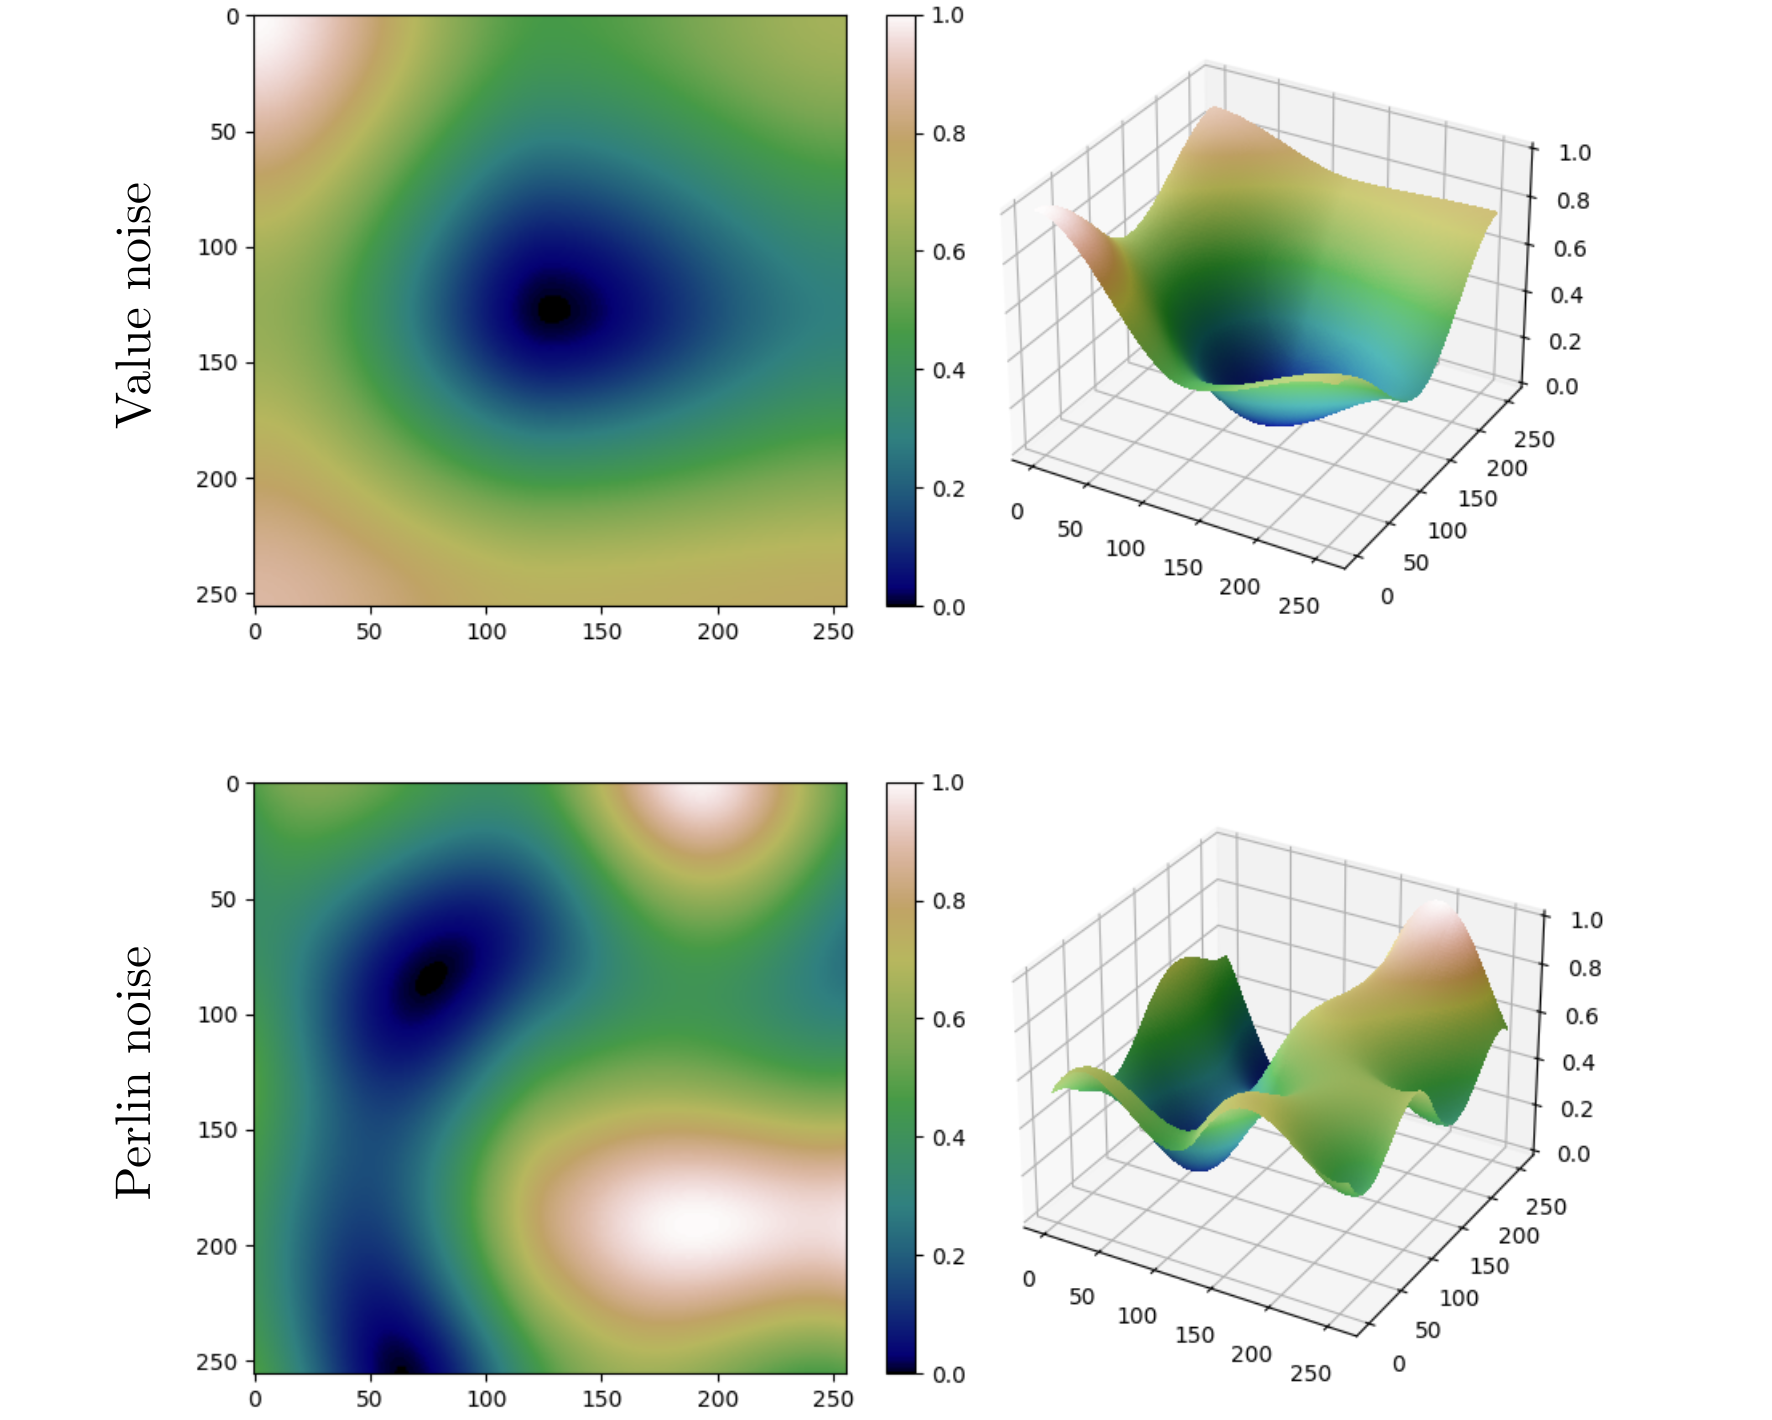
\includegraphics[width=\textwidth]{one layer noise.png}
    \caption{Single-octave Value and Perlin noise}
    \label{fig:single}
\end{figure}

As one may have noticed, since we have yet to add the fractal layers on this base layer, the terrain looks very artificial and unrealistic due to 
the overly smooth appearance. This is because a single-octave noise function lacks the high-frequency details and variation that give natural terrain 
its ruggedness and complexity. By introducing additional octaves through fractal summation, we can simulate the self-similar structure observed in 
real-world landscapes and significantly enhance visual realism. 

After calculating the remaining fractal layers, normalised height values were plottted on a 3D graph, resulting in Figure \ref{fig:plot_vf_pf}. 
\begin{figure}[H]
    \centering
    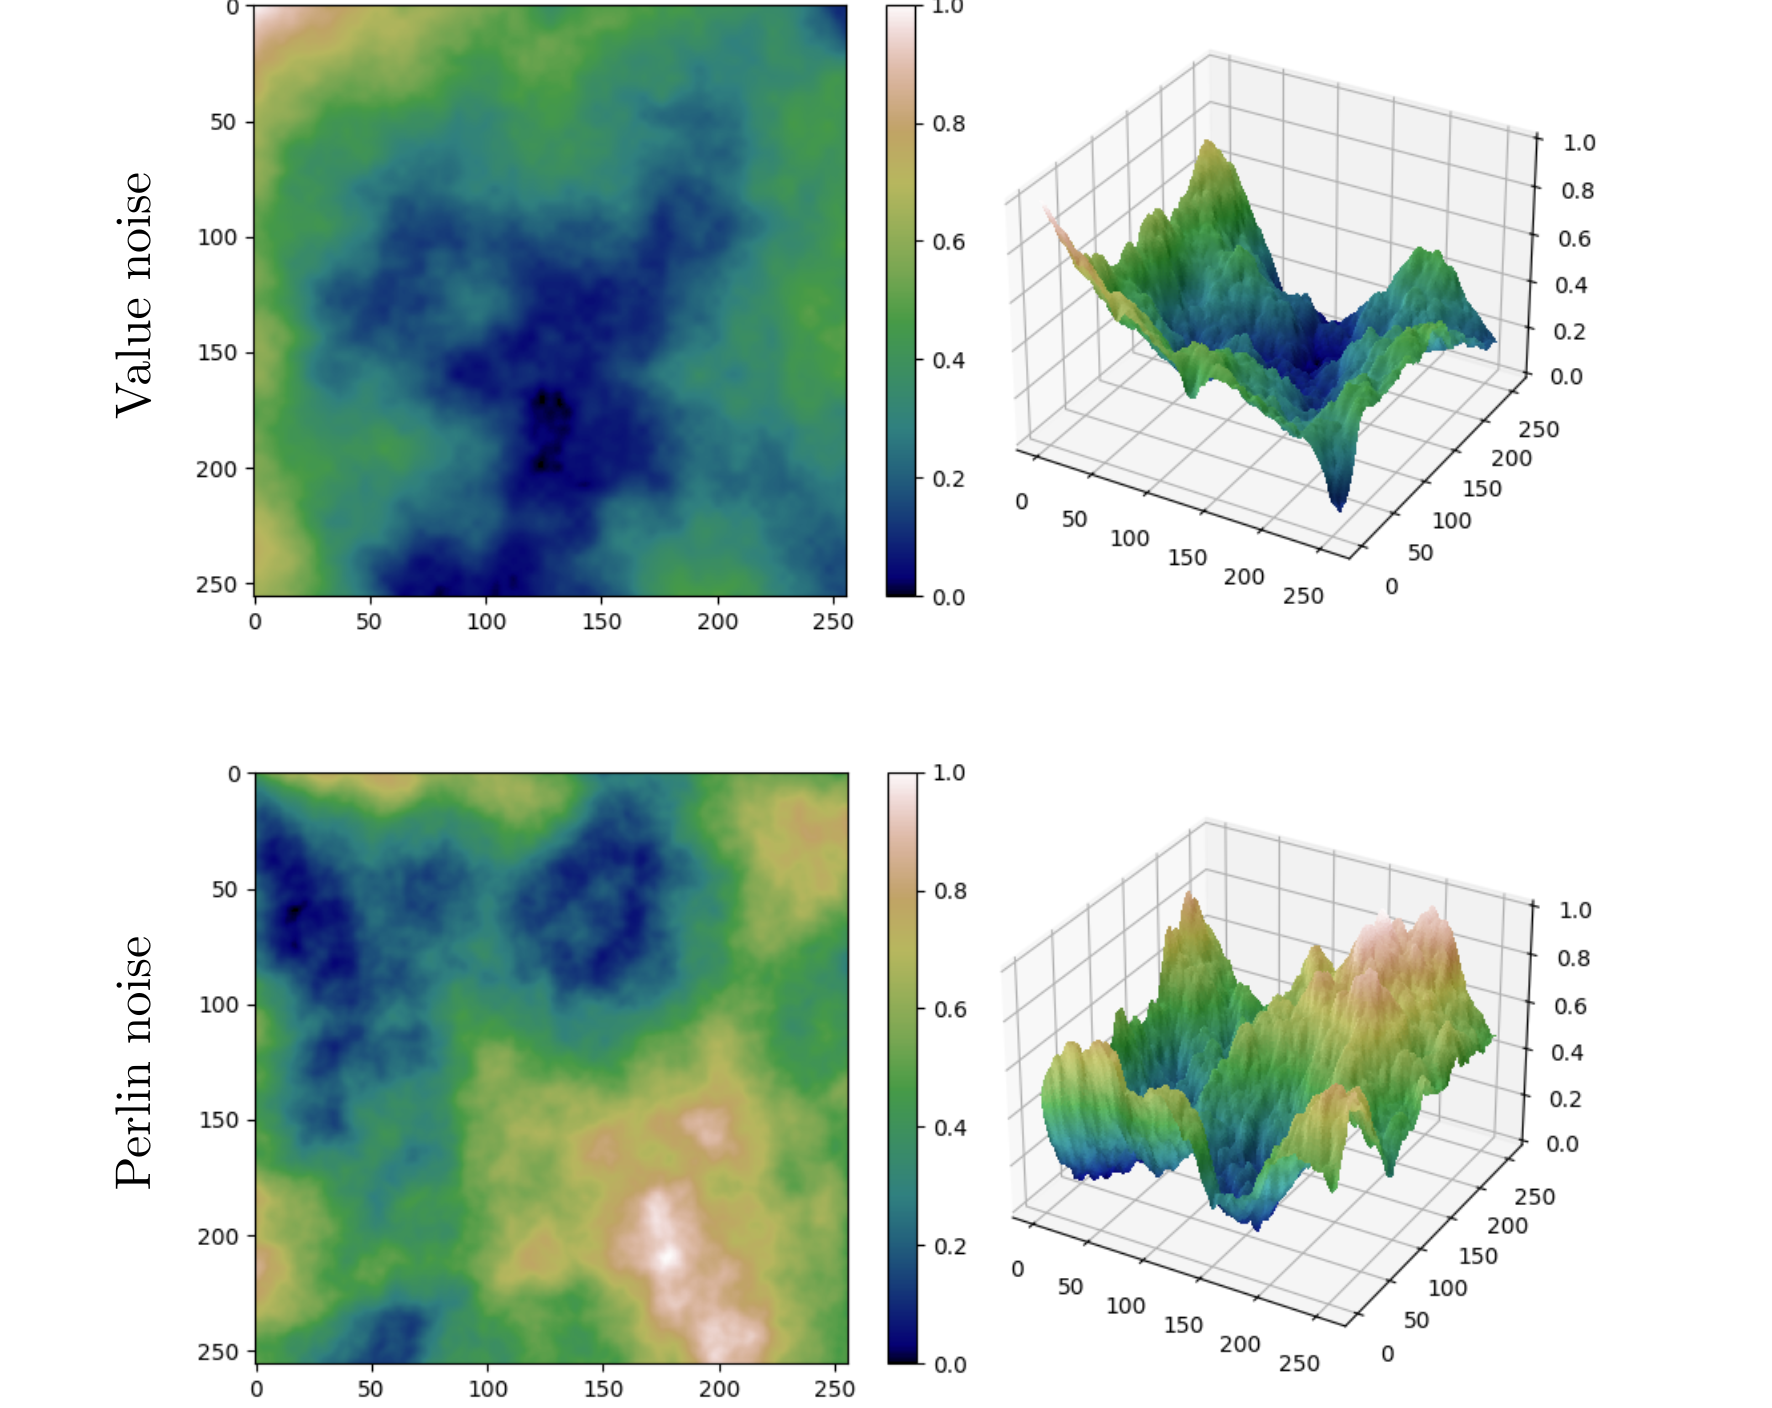
\includegraphics[width=\textwidth]{fractal noises.png}
    \caption{Plots of Value fractal noise and Perlin fractal noise}
    \label{fig:plot_vf_pf}
\end{figure}
We could see that this new terrain greatly enhance the quality of the terrain compared to Figure \ref{fig:single}. This is because each successive layer 
in a fractal noise adds finer detail (achieved through increasing the frequency) to the terrain while preserving the overall structure (by diminishing 
the amplitude of each layer) provided by the first layer. This multi-scale layering captures the hierarchical nature of natural topography, where broad 
mountain ranges coexist with smaller hills and surface irregularities.

After the calculations are completed, I now try to visually compare the Value noise and Perlin noise generated to assess which one produces an overall 
more realistic terrain.

\subsection{\textsc{Visual Comparison}}
\vspace*{-10pt}
The terrain output from Value noise and Perlin noise demonstrates fundamentally different characteristics when generated under identical parameters. 
The value noise terrain exhibits more broad and low-frequency features with fewer pronounced peaks. On the other hand, the Perlin noise terrain reveals 
a more “rugged” topology, characterized by the presence of higher frequency components such as sharper ridges and denser distribution of elevation extrema.  

While value noise is theoretically prone to producing artifacts due to its reliance on scalar interpolation between grid points, such artifacts are not 
prominently visible in the implementation due to the use of high-resolution grids. However, subtle evidence of value's noise limitations is still observable 
in Figure \ref{fig:limitations}, where certain regions appear to exhibit what may be interpreted as artifact-like features. For instance, the region near $(130,170)$ (Artifact 
zone 1, red box) shows an extreme lowland with steep boundaries. Likewise, this type of artifact with sudden changes in elevation can also be spotted near 
$(252,0)$ (Artifact zone 2, orange box). 

\begin{figure}[H]
    \centering
    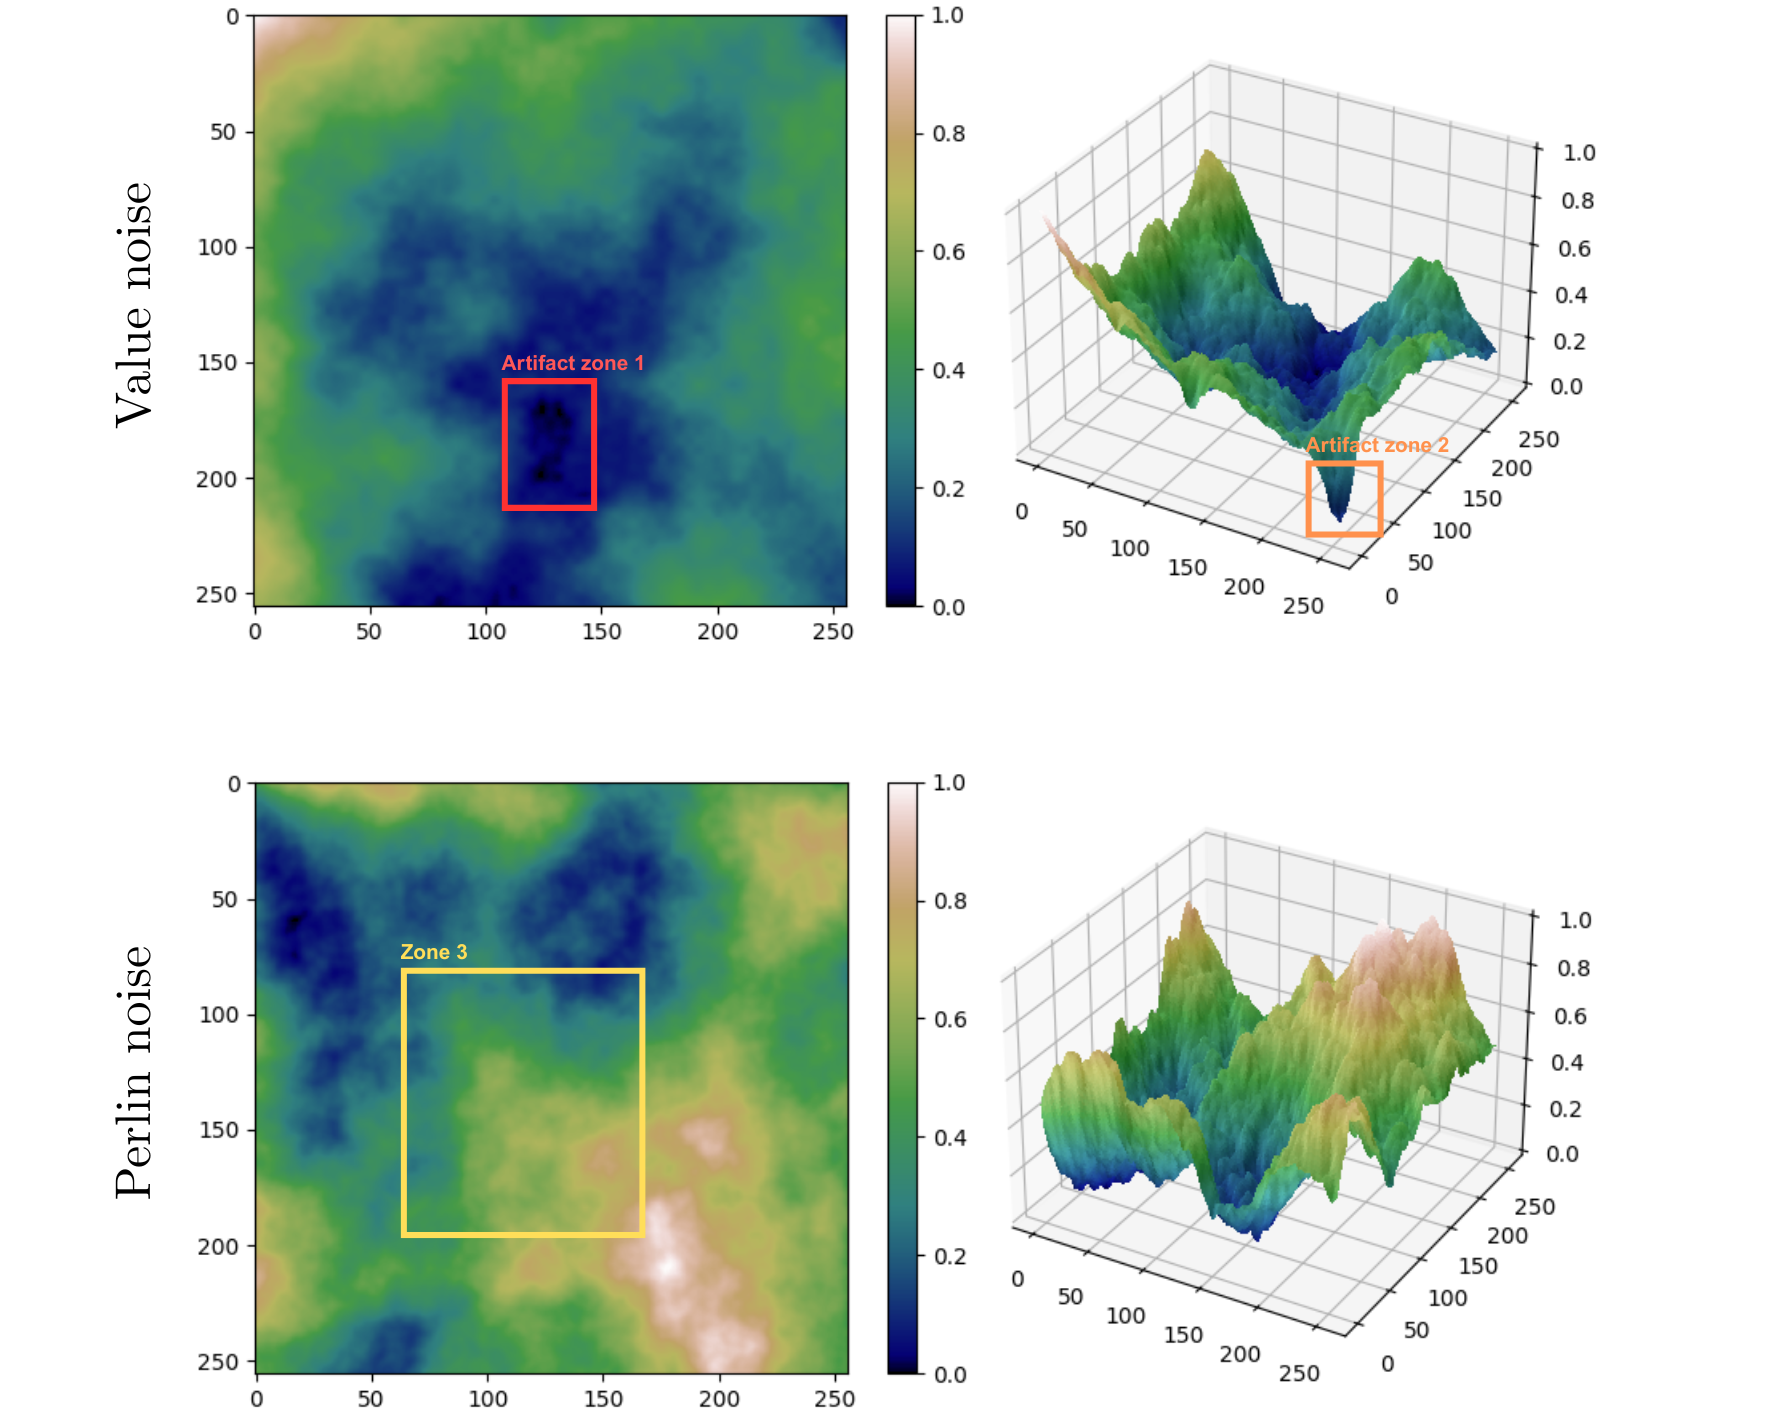
\includegraphics[width=\textwidth]{limitations.png}
    \caption{Visual comparisons, annotated from Figure \ref{fig:plot_vf_pf}, between the two noise types}
    \label{fig:limitations}
\end{figure}

In contrast, the Perlin noise terrain exhibits more continuous and coherent elevation transitions, evidenced by the smoother gradient from peaks to valleys (Zone 3, yellow box). 
This was achieved through gradient-based interpolation, which prevents the formation of artifacts as they are guided by the directional change of the terrain, 
not by flat scalar values. 

However, the distinction in realism is subtle and subjective, and thus these noises should be primarily evaluated with quantitative metrics mentioned in Section \ref{quant_metrics}. 

\subsection{\textsc{Quantitative Comparison}}
\vspace*{-10pt}

For a fair comparison, elevation data from GMTED2010 will first be resampled by taking a weighted average to the same size as the noise function $(256\times256)$, before normalizing 
to the range $[0,1]$. The geographic areas I have selected to compare the noise functions against can be seen in Table \ref{table:first_pick}.

\begin{table}[h!]
    \begin{tblr}{
        colspec={X[1.25,l] X[1.75,l] X[2.75,l] X[3,l]},
        width=\textwidth,
        hlines,
        row{1} = {gray9},
        rowsep=5pt,
    }
        \textbf{Region} & \textbf{Bounding box} & \textbf{Features} & \textbf{Test criteria} \\
        Swiss Alpes & 6.0°E-10.0°E, 45.5°N-47.5°N & pointy peaks and deep valleys & ability to create sharp ridges and smooth valley floors \\
        Himalayan Foothills & 85.0°E-87.0°E, 27.0°N-29.0°N & dense networks of parallel ridges and valleys & ability to produce organized, directional patterns \\
        Rocky Mountains & 7.65°E-7.70°E, 45.98°N-46.02°N & mix of rugged peaks and high flat plains & ability to blend steep slopes with gentle areas
    \end{tblr}
    \caption{Initial pick of geographical regions for quantitative comparisons}
    \label{table:first_pick}
\end{table}
\begin{figure}[H]
    \centering
    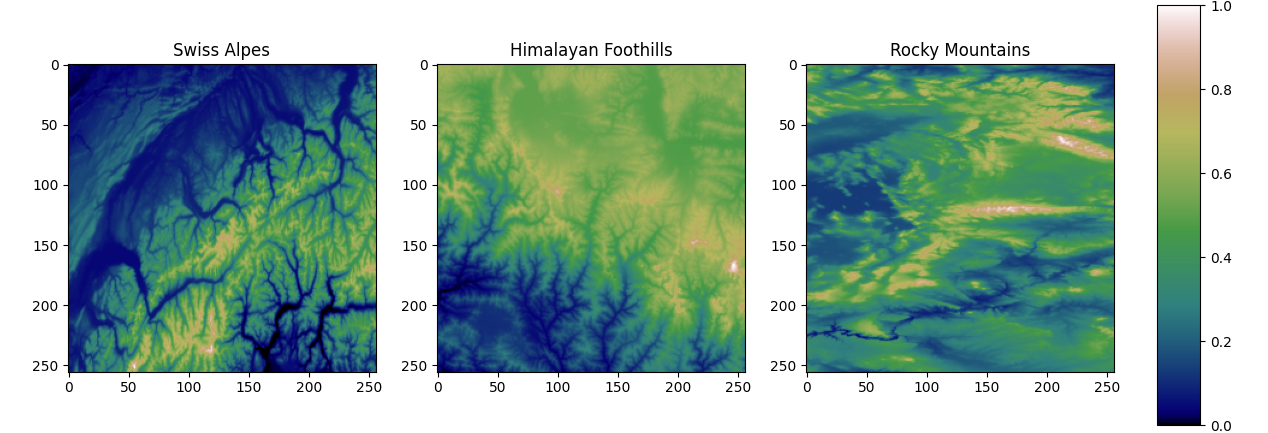
\includegraphics[width=\textwidth]{real data 2d.png}
    \caption{Initial real-life data plot}
    \label{fig:heatplot_realInit}
\end{figure}
The varied real-world terrains will ensure comprehensive evaluation of noise functions' ability to replicate elevation distribution statistics, spatial autocorrelation properties, 
and spectral properties.

However, when these terrains were plotted in Figure \ref{fig:heatplot_realInit}, it became apparent that my original selection of geographic regions needed to be reconsidered. The areas I had chosen spanned 
vast mountain ranges with highly complex and large-scale features. When these were down sampled to fit the $256\times256$ resolution required by my noise implementation, much of the detail 
and variability inherent to the original landscapes was lost. In contrast, my noise-generated terrains, constrained by both resolution and simplicity, tended to produce isolated 
mountainous forms rather than broad, interconnected ranges. Therefore, a new table of chosen geographic regions with scales more closely aligned with the spatial scope of my simulated 
terrains was created (Table \ref{table:final_pick}). 

\begin{table}[h!]
    \begin{tblr}{
        colspec={X[1.25,l] X[1.75,l] X[2.75,l] X[3,l]},
        width=\textwidth,
        hlines,
        row{1} = {gray9},
        rowsep=5pt,
    }
        \textbf{Region} & \textbf{Bounding box} & \textbf{Features} & \textbf{Test criteria} \\
        Everest & 86.9°E-87.0°E, 27.9°N-28.0°N & sharp peaks, deep valleys, extreme elevation gradients & ability to create sharp ridges and smooth valley floors \\
        Denali & 151.0°W-150.5°W, 63.0°N-63.2°N & parallel ridges from glacial flow & ability to produce directional patterns and consistent slope \\
        Matterhorn & 7.65°E-7.70°E, 45.98°N-46.02°N & mix of rugged peaks and gentle terrain & ability to have variations of features
    \end{tblr}
    \caption{Final pick of geographical regions for quantitative comparisons}
    \label{table:final_pick}
\end{table}
\begin{figure}[H]
    \centering
    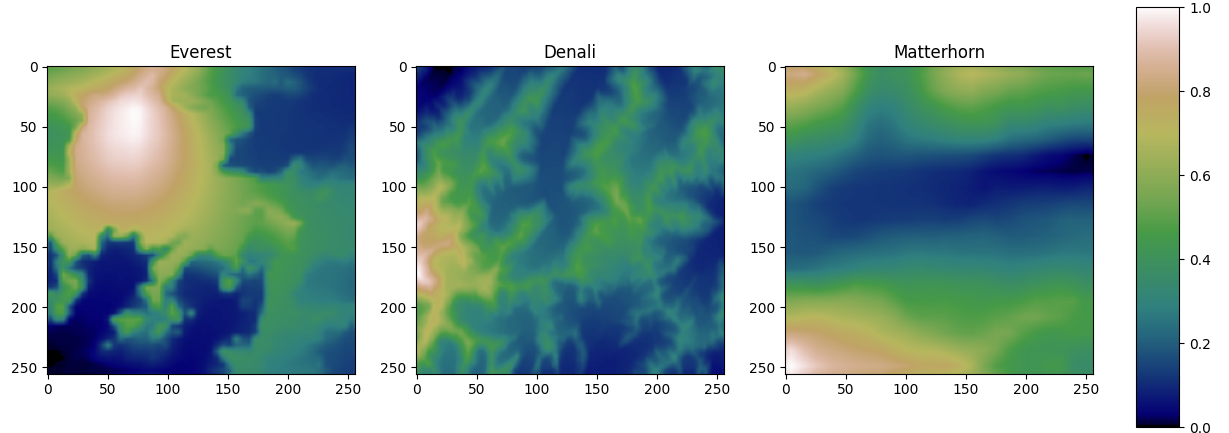
\includegraphics[width=\textwidth]{new real data 2D.png}
    \caption{Re-selected real-life data plot}
    \label{fig:heatplot_realFinal}
\end{figure}
Now that we have selected the terrain, I then use technology to compute the numerical statistical values listed in Section \ref{quant_metrics} for each of the 
real-life data. All of these results, rounded to 4 decimal places, are summarized in Table \ref{table:real_stats}.

\begin{table}[h!]
    \begin{tblr}{
        colspec={X[1,l] X[1,l] X[1,l] X[1,l] X[1,l] X[1,l] X[1,l]},
        width=\textwidth,
        hlines,
        row{1} = {gray9},
        rowsep=5pt,
    }
        \textbf{Region} & \textbf{Mean} & \textbf{Variance} & \textbf{Kurtosis} & \textbf{Skewness} & \textbf{TRI} & \textbf{Moran's I}\\
        Everest & 0.4071 & 0.0770 & -1.0391 & 0.4042 & 0.0086 & 0.9559 \\
        Denali & 0.2963 & 0.0260 & 1.7975 & 1.2217 & 0.0093 & 0.9205 \\
        Matterhorn & 0.3678 & 0.0443 & -0.4070 & 0.5347 & 0.0046 & 0.9833
    \end{tblr}
    \caption{Statistical measures of real-life data}
    \label{table:real_stats}
\end{table}

A histogram was also plotted and is shown here in Figure \ref{fig:histogram_real}

\begin{figure}[H]
    \centering
    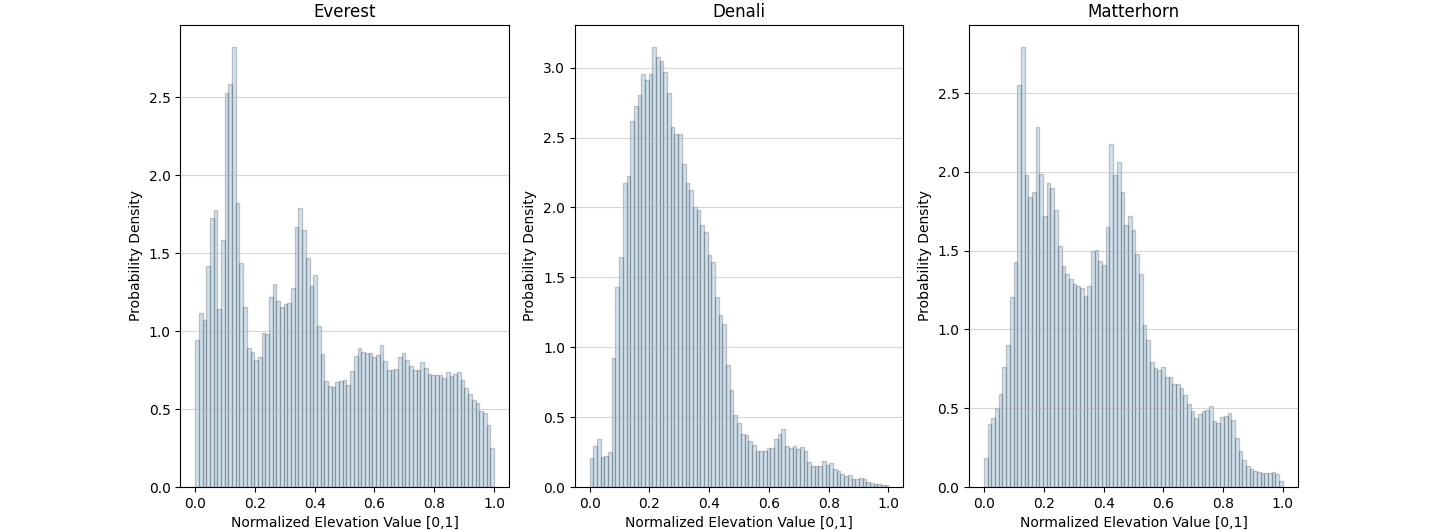
\includegraphics[width=\textwidth]{histogram real life data.png}
    \caption{Reselected real-life probability density histogram}
    \label{fig:histogram_real}
\end{figure}

Similarly, their Power Spectral Density was also computed and plotted in Figure \ref{fig:PSD_real}

\begin{figure}[H]
    \centering
    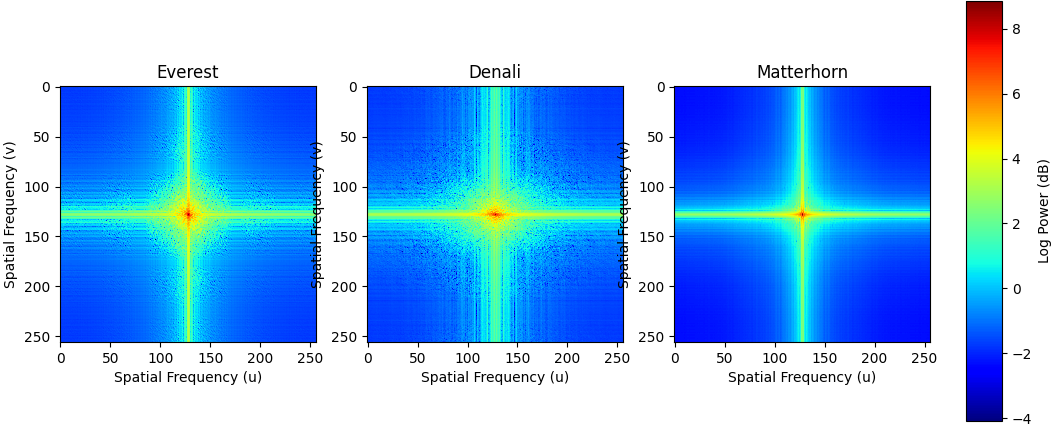
\includegraphics[width=\textwidth]{psd real life.png}
    \caption{PSD of the reselected real-life data}
    \label{fig:PSD_real}
\end{figure}

The mean elevation values obtained aligns with known elevation profiles, with Everest being the highest, followed by Matterhorn and Denali. The variance metric indicates Everest exhibits 
the most heterogeneous elevation distribution, consistent with its complex topography featuring dramatic shifts between high peaks and deep valleys as seen in Figure \ref{fig:heatplot_realFinal}. Denali's notably 
lower variance suggests more uniform elevation changes, while Matterhorn occupies the intermediate position. Kurtosis values reveal fundamentally different distribution shapes: Denali's 
positive kurtosis indicates leptokurtic distribution, suggesting concentrated elevation around the mean with extreme outliers with flatter terrain. In contrast, Everest and Matterhorn 
showed platykurtic distributions, implying more uniform elevation spread. Skewness values are universally positive, showing that all regions have more low-frequency features, though 
Denali's exceptionally high skewness showed disproportionate representation of lower elevations, which reflects its massive base compared to its summit. 

The Terrain Ruggedness Index (TRI) presents an interesting inversion, with Denali showing slightly greater roughness than Everest, despite Everest's higher variance. This suggests 
Denali's elevation changes are more locally concentrated, while Everest's variations are more globally distributed. Matterhorn's notably lower TRI indicates smoother transitions, 
consistent with its relatively uniform appearance in Figure \ref{fig:heatplot_realFinal}. Finally, Moran's I spatial autocorrelation values confirm strong elevation clustering, with Matterhorn exhibiting near-perfect 
spatial dependence. This is evident in that we can all clearly discern clusters of high elevation from clusters of low elevation. 

These statistical measures are corroborated by the PSD in Figure \ref{fig:PSD_real}. The PSD for Everest exhibits a broader spread of energy into the mid and high-frequency ranges, evident from the more 
diffused transition from red to green/blue. This aligns with Everest's high variance and kurtosis, reinforcing that Everest exhibit complex terrain morphology featuring both large scale 
elevation changes to fine-scale topographic details. For Denali, the PSD has a stronger central concentration of energy and a rapid falloff, signifying the dominance of low-frequency elements. 
This is also supported by the histogram (Figure \ref{fig:histogram_real}), which shows that there is little variation in the elevation data of Denali. Lastly, for Matterhorn, it retains a strong low-frequency core 
but with more pronounced mid-frequency components than Denali. This matches the intermediate variance and skewness in elevation distribution.

This quantitative analysis of Everest, Denali, and Matterhorn terrains establishes critical statistical benchmarks that will serve as essential reference points when evaluating noise-generated 
terrain models. The comprehensive statistical profiles reveal distinct yet consistent geomorphological signatures that must be replicated in synthetic terrains to achieve geological plausibility, 
particularly in their elevation distributions, topographic complexity, and spatial organization.

The parameters for the noise we will be using to compare will be the same as those used to generate Figure 5. Firstly, before comparing it to real-life elevation, I wanted to quantitively 
distinguish Perlin noise and Value noise. Like before, a table of statistical measures were calculated (Table \ref{table:noise_stats}), along with a histogram and the PSD. 

\begin{table}[h!]
    \begin{tblr}{
        colspec={X[1,l] X[1,l] X[1,l] X[1,l] X[1,l] X[1,l] X[1,l]},
        width=\textwidth,
        hlines,
        row{1} = {gray9},
        rowsep=5pt,
    }
        \textbf{Region} & \textbf{Mean} & \textbf{Variance} & \textbf{Kurtosis} & \textbf{Skewness} & \textbf{TRI} & \textbf{Moran's I}\\
        Value & 0.3041 & 0.0259 & 0.5373 & 0.6560 & 0.0065 & 0.9592 \\
        Perlin & 0.4542 & 0.0454 & -0.8280 & 0.1166 & 0.0101 & 0.9543
    \end{tblr}
    \caption{Statistical measures of noise-generated terrains}
    \label{table:noise_stats}
\end{table}

The synthetic elevation models generated using Noise and Perlin noise display distinct statistical and spatial characteristics. Perlin noise exhibits a higher mean elevation and nearly double 
the variance compared to pure Noise, indicating greater vertical heterogeneity and a broader distribution of elevation values. This aligns with the smoother yet more structured gradients typically 
associated with Perlin noise. The increased variance suggests that Perlin terrain incorporates more differentiated features, resembling the unevenness found in natural landscapes. In contrast, the 
lower variance in the Noise terrain reflects a more homogenous surface with minimal variation in elevation.

Kurtosis and skewness values further differentiate the two. The basic Value noise model yields a positive kurtosis, indicating a leptokurtic distribution with a sharper peak around the mean and 
more frequent extreme values. Perlin, by contrast, is distinctly platykurtic, suggesting a flatter distribution with fewer outliers and a more even spread of elevation values. This pattern is 
reinforced by skewness metrics: Value noise shows a strong positive skew, meaning lower elevation values dominate the distribution. Perlin's skewness is closer to zero, indicating a more symmetric 
terrain profile with less pronounced elevation bias.

The Terrain Ruggedness Index (TRI) again favors Perlin, although more subtly, with a slightly higher value compared to Value noise. While both values remain low relative to natural terrains, this 
suggests Perlin includes more local elevation changes and minor features that contribute to a more textured surface. Interestingly, Moran's I values remain high for both, indicating strong spatial 
autocorrelation. While this might be expected for Perlin due to its smooth gradients, the similarly high value for Noise implies that even the random noise used here exhibits spatial dependence, 
perhaps due to interpolation during generation.

Yet, when compared to the elevation profiles of real-world landscapes, both synthetic models exhibit a lack of realism. Starting with mean elevation, their modest averages reflect the absence of 
geological processes that typically generate both consistent patterns and extreme variations. Perlin noise, with its higher mean and smoother gradients, shows a weak resemblance to the balanced 
elevation profile of the Matterhorn. In contrast, Value noise, with its lower mean and more irregular characteristics, lacks similarity to any natural elevation structure.

In terms of variance, both models display a limited range, falling short of the broad elevation variability observed in real terrains. Even the Matterhorn, the least variable among the real-world 
examples, exhibits an order-of-magnitude greater heterogeneity. This suggests that neither synthetic model adequately captures the scale of variation resulting from processes such as tectonic 
uplift, erosion, or glacial carving. Although Perlin noise demonstrates a higher variance than Value noise, its fluctuations remain relatively subdued and fail to replicate the spatial intensity 
of natural landscapes.

Regarding kurtosis, Value noise presents a positive value that initially appears similar to Denali's. However, closer examination reveals that this similarity is likely superficial and the result 
of modeling artifacts. Perlin noise, on the other hand, exhibits negative kurtosis, showing a weak alignment with the profiles of Everest and the Matterhorn. Nevertheless, it still lacks the dynamic 
range and feature clustering, such as ridgelines, found in real terrain.

When skewness is considered, Value noise outperforms Perlin noise by favoring low-frequency elevation features. While this statistical resemblance may seem promising, it is important to note that 
natural skewness arises from geomorphological asymmetries not replicated in either model. As a result, the observed skewness in Value noise likely stems from randomness rather than an underlying 
structural basis.

Turning to the Terrain Ruggedness Index (TRI), both synthetic models produce values comparable to those of real-world terrains, indicating a degree of success in capturing fine-scale surface complexity. 
Furthermore, the Moran's I values of both noise types closely align with those of natural landscapes, suggesting that artificial noise functions are capable of mimicking spatial autocorrelation patterns 
found in nature.

\begin{figure}[H]
    \centering
    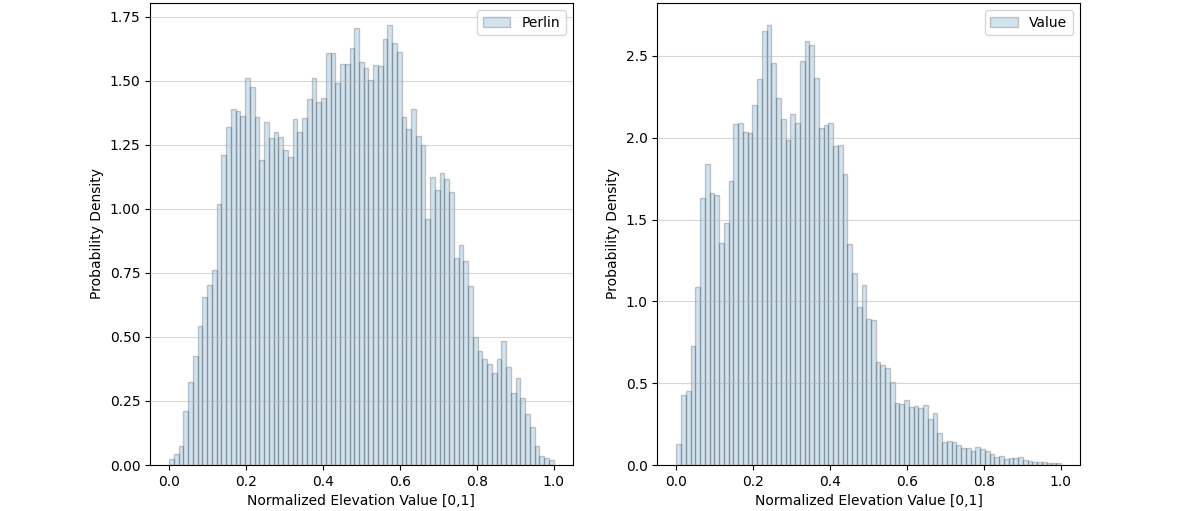
\includegraphics[width=\textwidth]{noise histogram.png}
    \caption{Noise terrain probability density diagram}
    \label{fig:histogram_noise}
\end{figure}

As illustrated in Figure \ref{fig:histogram_noise}, the probability density histogram indicates that Value noise more closely mirrors the elevation distribution observed in real terrains. However, histograms do not account for 
spatial arrangement or topographic continuity. Thus, while Value noise may approximate the statistical distribution of elevations, it still fails to replicate the structural coherence inherent to natural 
landscapes.

\begin{figure}[H]
    \centering
    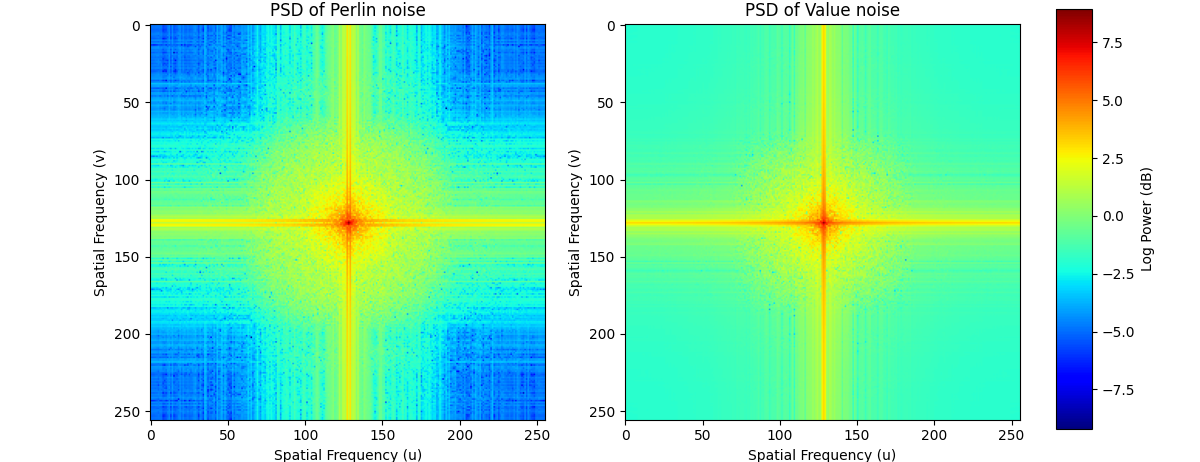
\includegraphics[width=\textwidth]{PSD noise.png}
    \caption{PSD of noise terrains}
    \label{fig:PSD_noise}
\end{figure}

Finally, as seen in Figure \ref{fig:PSD_noise}, The PSD of Perlin noise exhibits a pronounced concentration of energy at low spatial frequencies, visible as a bright central region that smoothly transitions into lower 
power at higher frequencies. This structure loosely resembles the PSDs of the real terrains, particularly Everest and Denali, which also display a central intensity peak with a radial decay, indicating 
a predominance of large-scale terrain features and a tapering of finer details. However, Perlin noise lacks the irregular frequency components evident in real terrains. Real landscapes such as Denali and 
Everest exhibit uneven, speckled distributions in the outer frequency bands, reflecting the complex, non-repeating, and multi-scale nature of geological formations. In contrast, Perlin noise displays a 
more symmetrical decay, characteristic of its algorithmic smoothness and periodicity.

On the other hand, the PSD of Value noise shows a far more uniform and flattened distribution compared to both Perlin noise and natural terrain. The concentration of power around the origin is less intense, 
and the surrounding frequency space remains relatively homogeneous, almost like white noise. Consequently, the Value noise PSD diverges considerably from the real terrain PSDs, where energy-rich low 
frequencies dominate. 
